\chapter{Máy trạng thái}

Máy trạng thái là một trong những những kĩ thuật lập trình mình gặp nhiều nhất khi lập trình nhúng, dường như nó xuất hiện ở khắp nơi. Nắm vững kĩ thuật này thì code các bạn viết sẽ trở nên mạch lạc, sáng sủa hơn, và việc đọc code của người khác trở nên đơn giản hơn.
\newpage

\section{Blocking vs. Non-blocking}

Blocking là gì? Hãy xem qua chương trình chớp tắt led trong Arduino như sau:
\begin{lstlisting}
void loop() {
  digitalWrite(LED_BUILTIN, HIGH);   
  delay(1000);                       
  digitalWrite(LED_BUILTIN, LOW);    
  delay(1000);                       
}
\end{lstlisting}

Có thể thấy là nó bật led, sử dụng hàm delay() trong 1 giây rồi tắt led, tiếp tục delay() và chương trình lặp lại liên tục.

Vấn đề là ở chỗ hàm delay(), chương trình đứng yên một chỗ và không làm gì cả, hay nói cách khác là nó bị \textbf{block} tại chỗ đó. Viết chương trình có chứa hàm tạm dừng một chỗ như delay() thì người ta gọi là \textbf{Blocking mode}. Trong thế giới nhúng, tài nguyên hạn chế nên chương trình đứng một chỗ như vậy là việc hết sức lãng phí. Thế nên có kiểu viết khác gọi là \textbf{Non-Blocking mode} nhằm làm cho chương trình chạy liên tục mà không bị đứng tại một điểm nào cả.

Ví dụ về viết kiểu Non-blocking cho chương trình chớp tắt led. Ý tưởng đằng sau này là lưu lại thời gian của lần bật/tắt led lần trước, rồi so sánh với thời điểm hiện tại, nếu nó vượt quá 1 giây chẳng hạn, thì tiến hành lần bật tắt tiếp theo.\newline

\begin{lstlisting}
void loop() {
    static uint32_t tick=0;
    static uint8_t led_state=LOW;
    if(millis()-tick>1000)
    {
        tick=millis();
        if(LOW==led_state){
            led_state=HIGH;
            digitalWrite(LED_BUILTIN, led_state);
        }
        else{
            led_state=LOW;
            digitalWrite(LED_BUILTIN, led_state);
        }
    }

    // Other code here
}
\end{lstlisting}

Như đoạn code trên, biến \textbf{tick} lưu lại thời gian của hoạt động bật/tắt led lần trước, lưu ý là nó phải được khai báo \textit{static} để không khởi tạo lại khi vòng loop bắt đầu vòng lặp mới.

Với cách viết như trên thì chương trình không bị đứng ở bất cứ điểm nào. Trong hàm loop(), chương trình liên tục hỏi đã đến lúc bật/tắt led hay chưa, nếu đến lúc thì thực hiện bật/tắt và lưu lại thời điểm vừa thực hiện. Nếu chưa thì thoát xuống làm chuyện khác. Đến đây bạn có thể viết chương trình điều khiển 2 led như sau:


Rồi đến đây thì bạn vừa có thể tiết kiệm được tài nguyên CPU, bằng cách làm nhiều tác vụ tuần tự nhau, vừa có thể thêm một số tính năng mới mà không cần phải đập đi xây lại, sugoi!!! Nhớ là mỗi tính năng bạn thêm vào đều phải đảm bảo tính Non-blocking he.
\section{Máy trạng thái}

Máy trạng thái (state machine) là thứ rất thường gặp trong lập trình nhúng. Ví dụ bạn viết chương trình điều khiển một cái động cơ, thì nó sẽ có những trạng thái như là đang dừng, đang quay ngược chiều hoặc cùng chiều kim đồng hồ... Máy trạng thái có thể hiểu là sơ đồ tất cả các trạng thái của một đối tượng nào đó và những điều kiện để chuyển từ trạng thái này sang trạng thái khác. Dưới đây là một ví dụ về chớp tắt led.
\begin{figure}[h!]
	\centering
\begin{tikzpicture}[->,>=stealth',shorten >=1pt,auto,node distance=5cm,
                    semithick]

  \node[initial,state] (A)                    	{$OFF$};
  \node[state]         (B) [right of=A] 		{$ON$};

  \path (A) edge [bend left]            node {500ms} (B)
        (B) edge [bend left]            node {500ms} (A);
 
\end{tikzpicture}
\caption{Chớp tắt led.}
\end{figure}

Đầu tiên bạn có thể thấy nó sẽ tắt led, và sau mỗi nửa giây nó lại đổi trạng thái một lần.

\section{Đặt vấn đề}

Bạn đang viết chương trình điều khiển xe mô hình, với chức năng tiến, lùi, quẹo phải, quẹo trái. Điều kiện của động cơ DC là khi đang quay sang phải thì không được quay sang trái ngay lập tức, mà phải dừng lại rồi mới được quay sang 

\begin{figure}[h!]
    \centering
    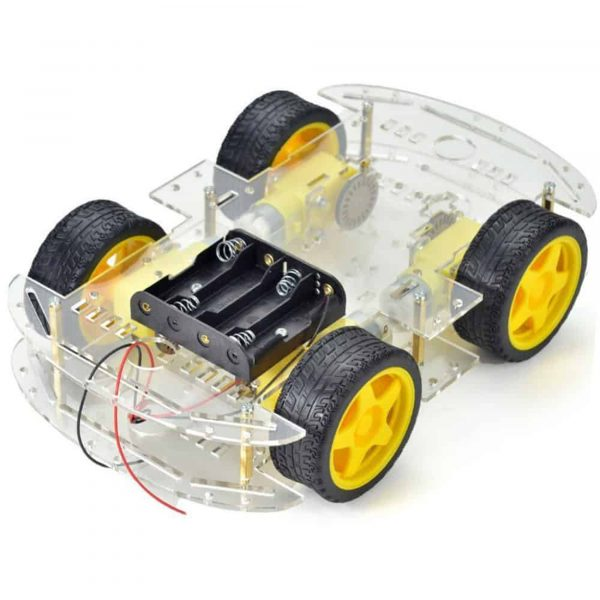
\includegraphics[width=0.8\linewidth]{images/xe_mo_hinh.jpg}
    \caption{Xe mô hình}
\end{figure}

